\section{A Synchronous Channel}

We now consider the implementation of a simple synchronous channel, extending
the trait in Figure~\ref{fig:SyncChanT}, using a JVM monitor.  Each
synchronisation goes through three stages, as represented in
Figure~\ref{fig:JVM-syncChan-seqDiagram}.
%
\begin{enumerate}
\item The sender  deposits its value, and signals to a receiver;

\item The receiver signals back to the sender, to provide a
  synchronisation, and returns the sender's value; 

\item The sender signals to a sender for the next synchronisation.
\end{enumerate}

%%%%%

\begin{figure}
\begin{center}
\def\height{5.2}
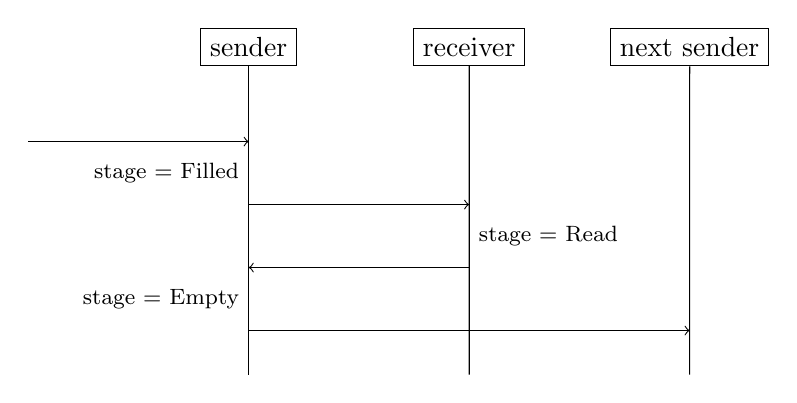
\begin{tikzpicture}[xscale = 2.8, yscale = 0.8]
\draw (0,0) node[draw] (sender) {sender};
\draw (sender) -- ++ (0,-\height);
\draw (1,0) node[draw] (receiver) {receiver}; 
\draw (receiver) -- ++ (0,-\height);
\draw (2,0) node[draw] (sender2) {next sender};
\draw (sender2) -- ++ (0,-\height);
%
\draw[<-] (sender) ++ (0,-1.5) --  ++ (-1,0); 
\draw (sender) ++ (0,-2.0) node[left]{\scalashape\footnotesize stage = Filled};
\draw[->] (sender) ++ (0,-2.5) --  ++ (1,0);
\draw (receiver) ++ (0,-3) node[right]{\scalashape\footnotesize stage = Read};
\draw[->] (receiver) ++ (0,-3.5) -- ++ (-1,0);
\draw (sender) ++ (0,-4.0) node[left]{\scalashape\footnotesize stage = Empty};
\draw[->] (sender) ++ (0,-4.5) -- ++ (2,0);
\end{tikzpicture}
\end{center}
\caption{A sequence diagram illustrating the signals in the implementation of
  a synchronous channel.}
\label{fig:JVM-syncChan-seqDiagram}
\end{figure}

%%%%%

The implementation in Figure~\ref{fig:JVM-SyncChan} uses a variable |value| to
store the sender's value.  It also uses a variable |stage| to record the
current stage of the synchronisation: whether |value| is (logically) empty,
has been filled, or  has been read by the receiver.

%%%%%

\begin{figure}
\begin{scala}
class JVMMonitorSyncChan[A] extends tacp.monitors.SyncChanT[A]{
  /** The current or previous value. */
  private var value = null.asInstanceOf[A]

  private val Empty = 0; private val Filled = 1; private val Read = 2

  /** The current stage of the exchange; is £value£ (logically) empty, has it been
    * filled, or has it been read by the receiver? */
  private var stage = Empty

  def send(x: A) = synchronized{
    while(stage != Empty) wait() // Wait for previous value to be consumed (1).
    value = x; stage = Filled   // Deposit my value.
    notifyAll() // Signal to receiver at (2).
    while(stage != Read) wait() // Wait for receiver (3).
    stage = Empty; notifyAll() // Signal to sender on next round at (1).
  }

  def receive(): A = synchronized{
    while(stage != Filled) wait() // Wait for sender (2).
    stage = Read; notifyAll()     // Notify current sender at (3).
    value
  }
}
\end{scala}
\caption{A synchronous channel.}
\label{fig:JVM-SyncChan}
\end{figure}

%%%%%

Threads have to wait in three different places: the sender has to wait for the
previous synchronisation to finish; the receiver has to wait for the sender to
deposit its value; and the sender has to wait for the receiver.  As we are
using a JVM monitor, we can't target the signals to the desired place.  We
therefore have to use |notifyAll| for each signal.  
Threads that receive the
signal can identify whether they should continue, or wait again, based on the
value of |stage|.
This is another example that works better with SCL |Condition|s, allowing
signals to be targeted.


\begin{instruction}
Study the details of the implementation.
\end{instruction}

%%%%%%%%%%%%%%%%%%%%%%%%%%%%%%%%%%%%%%%%%%%%%%%%%%%%%%%

\section{A Barrier Synchronisation Object}

%%%%%

\begin{figure}[btp]
\begin{scala}
class JVMMonitorBarrier(n: Int) extends BarrierT{
  /** The number of threads currently waiting. */
  private var count = 0

  /** Are we in the leaving phase of a synchronisation? */
  private var leaving = false

  def sync(me: Int) = synchronized{
    while(leaving) wait() // Wait for previous synchronisation to end (1).
    if(count == n-1){      // Start leaving phase
      leaving = true; notifyAll() // Signal to threads at (2).
    }
    else{      // Have to wait
      count += 1
      while(!leaving) wait() // Wait for the others (2).
      count -= 1
    }
    if(count == 0){      // Start entering phase.
      leaving = false; notifyAll() // Signal to threads at (1).
    }
  }
} 
\end{scala}
\caption{A barrier synchronisation object.}
\label{fig:JVMMonitorBarrier}
\end{figure}

%%%%%

We now consider a barrier synchronisation object.  The implementation is in
Figure~\ref{fig:JVMMonitorBarrier}.  It is a fairly straightforward adaptation
of the implementation using |Condition|s, from
Figure~\ref{fig:ConditionsBarrier}.  The variable |leaving| records whether
the object is in the leaving |phase| of a synchronisation.  The variable
|count| records how many threads are waiting during the entering phase, and
how many still need to leave during the leaving phase.

Each thread waits at point (1) in the code, until the previous synchronisation
is complete.  Subsequently, the first $\sm n -1$ threads wait at point~(2) for
the other threads.  The |n|th thread starts the leaving phase, and signals to
the other threads.  The last thread to leave starts the entering phase of the
next synchronisation, and signals to the waiting threads at point~(1).

\begin{instruction}
Study the details of the implementation.
\end{instruction}

Suppose the barrier synchronisation is used by exactly |n| threads, as is the
usual case.  Then we can never have threads waiting at both points~(1) and~(2)
simultaneously: threads wait at~(1) only during the leaving phase, and threads
wait at~(2) only during the entering phase.  This means that each |notifyAll|
wakes up only the intended threads.  Of course, the threads still need to
recheck the relevant condition when they do awake, to guard against spurious
wakeups.

%%%%%%%%%%%%%%%%%%%%%%%%%%%%%%%%%%%%%%%%%%%%%%%%%%%%%%%

\section{A Timeout Exchanger}
\label{sec:timed-exchanger}

In previous chapters, we saw a couple of implementations of an exchanger: an
object that allows two threads to swap values of some type~|A|.  In this
section we consider an exchanger with a timeout: if a thread fails to exchange
within some period of time, it will timeout and fail.  We will also allow the
exchange to fail under another couple of circumstances, which we discuss below.

In order to capture the possibility of failure, we give the |exchange|
operation the following signature:
%
\begin{scala}
  def exchange(x: A): Option[A]
\end{scala}
% 
A return value of |Some(y)| will indicate that the thread has successfully
exchanged with another thread and obtained~|y|; a return value of |None| will
indicate that the exchange failed. 

In order to implement the timeout, we will need another form of the |wait|
operation.  The operation |wait(delay)| is like a standard |wait()|, except if
it doesn't receive a signal, it will timeout after |delay| milliseconds (ms).
In each case, the thread needs to then wait to reobtain the lock on the
monitor.  The client code is responsible for working out whether it received a
signal or not.

There is another version, |wait(millis, nanos)|, which waits for |millis|
milliseconds and |nanos| nanoseconds (ns); equivalently, it waits for
$1,000,000 \times \sm{millis} + \sm{nanos}$\,ns.  

A millisecond is rather a long time for a thread to wait for another thread.
(Delays measured in milliseconds might be appropriate to wait for a human or
for a network communication.)  We therefore use this latter form, and measure
the timeout time for the exchanger in nanoseconds.  The class has an |Int|
parameter |delay| that defines the delay, so the maximum delay will be
|Int.MaxValue| $= 2^{31}-1$\, ns, about two seconds.

Our implementation is in Figure~\ref{fig:TimeoutExchanger}.  It is somewhat
similar to the exchanger in Figure~\ref{fig:MonitorExchanger}.  It uses a
variable |stage| that records which stage has been reached.  This variable
will store one of the following values.
%
\begin{description}
\item[{\scalastyle Empty}:] No thread is currently exchanging;

\item[{\scalashape Filled}:] The first thread has deposited its value;

\item[{\scalashape Exchanging}:] An exchange is underway: the second thread
  has taken the first thread's value, and swapped it with its own value.
\end{description}


%%%%%

\begin{figure}
\begin{scala}
class TimeoutExchanger[A](delay: Int){
  private var slot: A = _

  private val Empty = 0; private val Filled = 1; private val Exchanging = 2

  private var stage: Int = Empty

  def exchange(x: A): Option[A] = synchronized{
    if(stage == Empty){
      // Deposit my value and wait.
      slot = x; stage = Filled; wait(0, delay)
      if(stage == Exchanging){ stage = Empty; Some(slot) } // Success.
      else{ assert(stage == Filled); stage = Empty; None } // No joy.
    }
    else if(stage == Filled){  // Take value in £slot£; deposit my value there.
      val result = slot; slot = x; stage = Exchanging; notify(); Some(result)
    }
    else{ assert(stage == Exchanging); None } // Another exchange is under way.
  }
}
\end{scala}
\caption{A timeout exchanger.}
\label{fig:TimeoutExchanger}
\end{figure}

%%%%%

If a thread finds that $\sm{stage} = \sm{Empty}$, it is the first thread in
the exchange.  It stores its value, sets $\sm{stage} = \sm{Filled}$, and waits
for up to |delay|\,ns.  When it wakes up, if $\sm{stage} = \sm{Exchanging}$,
another thread has deposited a value, so it can return that value, resetting
for the next round.  In fact, it acts the same way if it times out just before
another thread deposits its value; this behaviour seems appropriate.
Alternatively, if it finds that |stage| is still |Filled| when it wakes up, it
has failed to exchange, so resets for the next stage, and returns |None|.
This latter behaviour would also result from a spurious wakeup; we consider
this behaviour acceptable: to detect the spurious wakeup would require
comparing the system time before and after the |wait|, which is awkward.

If the thread initially finds that $\sm{stage} = \sm{Filled}$, it is the
second thread in the exchange.  It swaps its value with the value stored by
the first thread, sets |stage| to |Exchanging|, signals to the first thread,
and returns the first thread's value. 

If the thread initially finds that $\sm{stage} = \sm{Exchanging}$, it means
that two other threads are currently exchanging.  Clearly, this thread should
not interfere with that exchange.  We make the decision to treat this case as
a failure to exchange, and just return |None|.  An alternative would be to
wait while $\sm{stage} = \sm{Exchanging}$, for up to |delay|\,ns.  If
subsequently this thread becomes the first thread in an exchange, the length
of its subsequent wait would have to be adjusted based on the length of the
earlier wait.  This is rather messy, so we don't adopt this approach. 

\begin{instruction}
Study the details of the implementation.
\end{instruction}

The timeout exchanger can be tested much the same as the basic exchanger in
Section~\ref{sec:exchanger}, except we should also allow an attempted exchange
to fail.  Note that we cannot require an attempted exchange to succeed, even
if it overlaps in time with another attempt: it is possible that unfortunate
scheduling means that one of the threads is delayed, so as to prevent the
exchange.
